\documentclass{article}

\usepackage{arxiv}

\usepackage[utf8]{inputenc} % allow utf-8 input
\usepackage[T1]{fontenc}    % use 8-bit T1 fonts
\usepackage{hyperref}       % hyperlinks
\usepackage{url}            % simple URL typesetting
\usepackage{booktabs}       % professional-quality tables
\usepackage{amsfonts}       % blackboard math symbols
\usepackage{nicefrac}       % compact symbols for 1/2, etc.
\usepackage{microtype}      % microtypography
\usepackage{cleveref}       % smart cross-referencing
\usepackage{lipsum}         % Can be removed after putting your text content
\usepackage{graphicx}
\usepackage{natbib}
\usepackage{doi}

\title{A template for the \emph{arxiv} style}

% Here you can change the date presented in the paper title
%\date{September 9, 1985}
% Or remove it
%\date{}

\newif\ifuniqueAffiliation
% Comment to use multiple affiliations variant of author block 
\uniqueAffiliationtrue

\ifuniqueAffiliation % Standard variant of author block
\author{ \href{https://orcid.org/0000-0000-0000-0000}{
\includegraphics[scale=0.06]{orcid.pdf}\hspace{1mm}David S.~Hippocampus}\thanks{Use footnote for providing further
		information about author (webpage, alternative
		address)---\emph{not} for acknowledging funding agencies.} \\
	Department of Computer Science\\
	Cranberry-Lemon University\\
	Pittsburgh, PA 15213 \\
	\texttt{hippo@cs.cranberry-lemon.edu} \\
	%% examples of more authors
	\And
	\href{https://orcid.org/0000-0000-0000-0000}{
\includegraphics[scale=0.06]{orcid.pdf}\hspace{1mm}Elias D.~Striatum} \\
	Department of Electrical Engineering\\
	Mount-Sheikh University\\
	Santa Narimana, Levand \\
	\texttt{stariate@ee.mount-sheikh.edu} \\
	%% \AND
	%% Coauthor \\
	%% Affiliation \\
	%% Address \\
	%% \texttt{email} \\
	%% \And
	%% Coauthor \\
	%% Affiliation \\
	%% Address \\
	%% \texttt{email} \\
	%% \And
	%% Coauthor \\
	%% Affiliation \\
	%% Address \\
	%% \texttt{email} \\
}
\else
% Multiple affiliations variant of author block
\usepackage{authblk}
\renewcommand\Authfont{\bfseries}
\setlength{\affilsep}{0em}
% box is needed for correct spacing with authblk
\newbox{\orcid}\sbox{\orcid}{
\includegraphics[scale=0.06]{orcid.pdf}} 
\author[1]{%
	\href{https://orcid.org/0000-0000-0000-0000}{\usebox{\orcid}\hspace{1mm}David S.~Hippocampus\thanks{\texttt{hippo@cs.cranberry-lemon.edu}}}%
}
\author[1,2]{%
	\href{https://orcid.org/0000-0000-0000-0000}{\usebox{\orcid}\hspace{1mm}Elias D.~Striatum\thanks{\texttt{stariate@ee.mount-sheikh.edu}}}%
}
\affil[1]{Department of Computer Science, Cranberry-Lemon University, Pittsburgh, PA 15213}
\affil[2]{Department of Electrical Engineering, Mount-Sheikh University, Santa Narimana, Levand}
\fi

%%% Add PDF metadata to help others organize their library
%%% Once the PDF is generated, you can check the metadata with
%%% $ pdfinfo template.pdf
\hypersetup{
pdftitle={A template for the arxiv style},
pdfsubject={q-bio.NC, q-bio.QM},
pdfauthor={David S.~Hippocampus, Elias D.~Striatum},
pdfkeywords={First keyword, Second keyword, More},
}

\begin{document}
\maketitle

\begin{abstract}
    Recent advancements in mobile and positioning technologies have revolutionised mobility studies, enabling researchers to analyse large-scale movement data with high spatial and temporal resolution. This has many significant real-world implications spanning urban planning, transportation network design, disease spread modelling, and understanding socio-economic segregation patterns.
    Stop location detection belongs to this realm, however, while significant advancements have been made in mobility studies, it remains a relatively understudied area within this field. Existing methods, often based on density clustering algorithms, face challenges in handling noisy data and identifying isolated stop points.
    This paper proposes a classification algorithm that builds upon density-based methods to detect stop positions. The algorithm integrates various features, including individual routines, collective behaviour, and external factors. By considering collective information, the method aims to overcome the limitations of incomplete individual data and identify non-routine stop locations.
    The proposed approach addresses the inherent noise in mobility data and offers a comprehensive solution for accurate stop detection. It considers external factors such as holidays, period of the day and day of the week, which can influence movement decisions or leverage on routine patterns. 
    % something about the conclusion and the results? 
\end{abstract}


% keywords can be removed
\keywords{urban mobility, stop location detection, collective behaviour}
%to check

%Participants in Alphabetical Order + Tutors at the end

\section{Introduction}
%~\cite{Massimiliano2021} weather and presence of city events as features in DL to predict human mobility
%~\cite{Ramaswamy2004} Project Lachesis: Parsing and Modeling Location Histories with DBSCAN algorithm
%~\cite{Aslak2020} Infomap finds destination aggregating individual stays without using DBSCAN to for multi-user traces, when individuals share many destinations
%Something about big data and so on

The advent of mobile devices and positioning technologies in recent decades has renewed scientific interest in mobility studies, enabling the inference of trajectories from sources like mobile phone logs, social network data, and GPS records. Researchers now leverage large-scale datasets from electronics, media, telecommunications companies, and experimental studies to analyze the movements of millions of individuals over extensive periods with high spatial and temporal resolution. Understanding human mobility is crucial for addressing real-world challenges related not only to urban planning studies~\citep{DeNadai2016}, the design of efficient transport networks~\citep{Ferretti2018} and sustainable cities~\citep{Caitlin2015}. In particular, it has proved to be instrumental in understanding the spread of diseases~\citep{Moritz2020, Oliver2020, Aguilar-Sanchez2022, klein2023forecasting} and socio-economic segregation~\citep{Pappalardo2015, Centellegher2024}.

Stop location detection, a crucial process in individual mobility studies, enables the analysis of personal habits and community-wide patterns. Despite its importance, this area has received comparatively less attention than trajectory reconstruction research~\citep{Ramaswamy2004, Aslak2020}. The challenge is further complicated by the inherent noise in mobility data, presenting a significant obstacle to accurate detection methods.

Previous research on trajectory data can be broadly categorized into two main approaches: mining important places using multiple trajectories and extracting interesting sequences from single trajectories. For single trajectory analysis, traditional methods often rely on movement parameters like speed and direction to segment trajectories and identify stops.

Density-based clustering algorithms, such as DBSCAN (Density-Based Spatial Clustering of Applications with Noise) \citep{ester1996density} and OPTICS (Ordering Points To Identify the Clustering Structure) \citep{ankerst1999optics}, have inspired numerous applications in this field. These algorithms utilize concepts like density reachability to identify clusters, requiring parameters such as maximum radius and minimum points to form a cluster.

Several clustering-based methods have been developed specifically for stop extraction. CB-SMoT (Clustering-Based Stop and Move of Trajectories) \citep{palma2008clustering} extends DBSCAN by incorporating average speed but struggles with stops containing few slow points. T-OPTICS (Trajectory-OPTICS) \citep{zimmermann2009finding} adapts the OPTICS framework but focuses solely on proximity without considering duration. TrajDBSCAN (Trajectory DBSCAN) \citep{tran2011robust} uses geographical distance instead of travel distance, making it less sensitive to speed variations, but still faces challenges with noisy trajectories.
These existing methods have limitations in handling noisy data, identifying isolated stop points with large time intervals, and merging noise-interrupted sequences into stops. Additionally, trajectory segmentation approaches like those proposed by Buchin et al. \citep{buchin2011segmenting} and Junior et al. \citep{soares2015grasp} offer alternative perspectives but give little attention to noise in trajectories.

One of the most widely adopted methods, known as Project Lachesis~\citep{Ramaswamy2004} relies on density-based principles and initially filters out non-stationary positions and subsequently clusters nearby points within a specified radius and time interval using DBSCAN.
More recently,~\citep{Aslak2020} introduced Infostop, building upon similar filtering techniques to employ the network community detection algorithm Infomap to identify destination points for each individual even for multi-user traces.
Narrowing the focus solely to the individual level may pose risks due to the inherent noise or missing data in GPS records which can suffer from spatial and temporal gaps. Therefore, even when individual-level data is incomplete or inaccurate, it is critical to use methods that can reliably detect stop locations.

To address this challenge, our proposed classification algorithm works on top of a density based method in order to detect stop positions by integrating various features, incorporating not only individual routines but also considering collective perspectives and external factors that may influence the location of stopping points.
Taking into account collective behavioural information can be instrumental in filling in the gaps caused by missing individual data, and can also provide insights into identifying stop positions outside of an individual's routine~\citep{Bontorin2024a}.
Further, external factors such as weather conditions or holiday days can influence the decisions~\citep{Massimiliano2021}.


% noise in the data, need to spot stop points even with slightly different positions (low precision). Problem of missing data
% main state of the art based on density based model~\cite{Ramaswamy2004}.
%Infomap propose a different way of aggregating~\cite{Aslak2020}  to for multi-user traces, when individuals share many destinations
% importance of consider together indiviual and collective trend to guess the missing data
%Taking into account collective behavioural information can be instrumental in filling in the gaps caused by missing individual data, and can also provide insight into identifying stop positions outside of an individual's routine~\citep{Bontorin2024a}.
% add other features that can be useful \cite{Massimiliano2021} weather and presence of city events as features in DL to predict human mobility
% differences with Infomap: we add other features and we consider collective and individual behaviour together. This can help in case of missing or noisy data.




\section{Methods}
\label{sec:methods}
% Machine learning algorithm to include different features such as collective and individual behaviour, tailoring it according to the period of the day, and the day of the week. We also consider the history of the individual in the previous week to get the recent trend at the individual level.
% We are working at geohash level at level 7, which means an area of about  153 m X 153 m.

%Describe the problem
% we include users in our panel who were active since February 1, 2024, were active for at least 21 days per month between February and March, 2024, generated at least one location ping per hour, on average
\subsection{Data description}
The data is provided by Cuebiq Inc. through their Data for Good initiative\footnote{\url{https://www.cuebiq.com/about/data-for-good/}}.
The dataset comprises privacy-enhanced (through up-leveling and aggregation) GPS locations, covering the period from February 2024 to March 2024 in the Core-based statistical area (CBSA) of New York-Newark-Jersey City, NY-NJ-PA MSA. Following the approach adopted by Klein et al.~\citep{Klein2023} to ensure data quality, we included only users active from February 1, 2024, participating for at least 20 days per month between February and March 2024, and generating at least 200 location ping per day on average. This filtering resulted in 2732 devices being included in the dataset. This dataset includes only users who voluntarily opted to share their data anonymously. To enhance and maintain user privacy, sensitive locations such as home and work are obfuscated to the Census Block Group level. The data collection process utilizes the Cuebiq Software Development Kit (SDK), which gathers user locations via GPS and Wi-Fi signals from Android and iOS devices.
% Plot with some descriptive statistics of data
For the geographic aggregation of points, we employ geohashs, a hierarchical spatial data structure that encodes locations using alphanumeric strings. This system subdivides geographic space into grid-shaped buckets, with the precision of the location increasing proportionally to the length of the geohash string. This method allows for efficient spatial indexing and aggregation of our dataset while maintaining adjustable levels of geographic precision.
Our data is collected at various geohash levels, with the highest level being up to level 9 depending on the device.
For our analysis, we aggregate the data to geohash level 8,  An 8-character geohash is approximately 25m×5m in size, which may vary based on region on the globe (e.g., 38m×19m at the equator~\citep{geohash})

Each point is characterized by a unique ID associated with the device, geographical coordinates and geohash of its position, and a timestamp.
To evaluate the robustness of our stop detection model in the presence of data gaps, we implemented a synthetic data reduction process on top of a sequence-oriented and density-based stop detection algorithm. This approach allows us to simulate real-world scenarios where data may be incomplete or missing.


Our dataset comprises individual location pings, each annotated with labels indicating whether they were identified as part of a stop by the sequence-oriented and density-dependent algorithm. To simulate temporal and spatial gaps in the data, we systematically removed the entire point cloud for 10\% of the detected stops, retaining only two points from each of these stops. This data reduction process was conducted with consideration for several factors, including device persistence, geohash type, stop classification given by the device traffic in that area, and day of the week.
This synthetic data manipulation serves two purposes: first, it allows us to assess the performance of our model under conditions of data sparsity, and second, it provides a controlled environment to compare our method against existing approaches that may be less robust to missing data.
%Additional information is included to characterize the geographical point or assess the reliability of the device.
%make reference to the images

To display the temporal patterns in the data,  Figure~\ref{fig:fig_trend} shows the daily number of unique devices and stops for the entire study period. From the geographical perspective, in Figure~\ref{fig:fig_geohash_heatmap}, we report the number of stops at the geohash level. 

\begin{figure}[ht]
    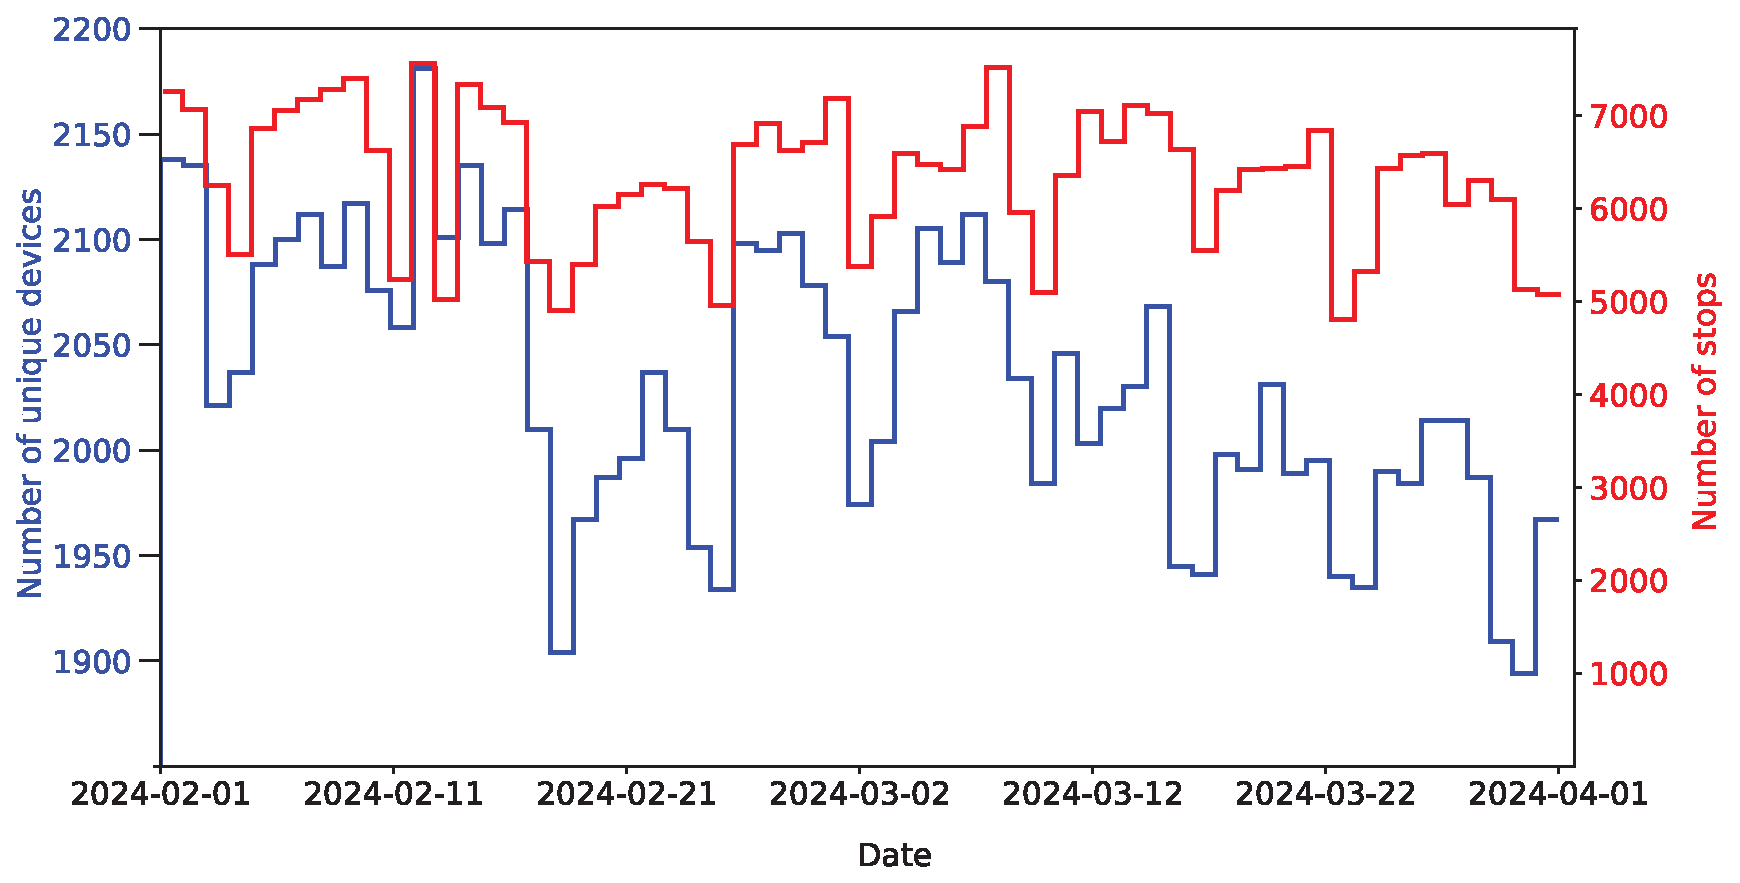
\includegraphics[width=0.8\textwidth]{./Images/figure_trends.eps}
	\centering
	%\fbox{\rule[-.5cm]{4cm}{4cm} \rule[-.5cm]{4cm}{0cm}}
	\caption{Daily trends showing the number of unique devices (blue line) and the number of stops (red line).}
	\label{fig:fig_trend}
\end{figure}

\begin{figure}[ht]
    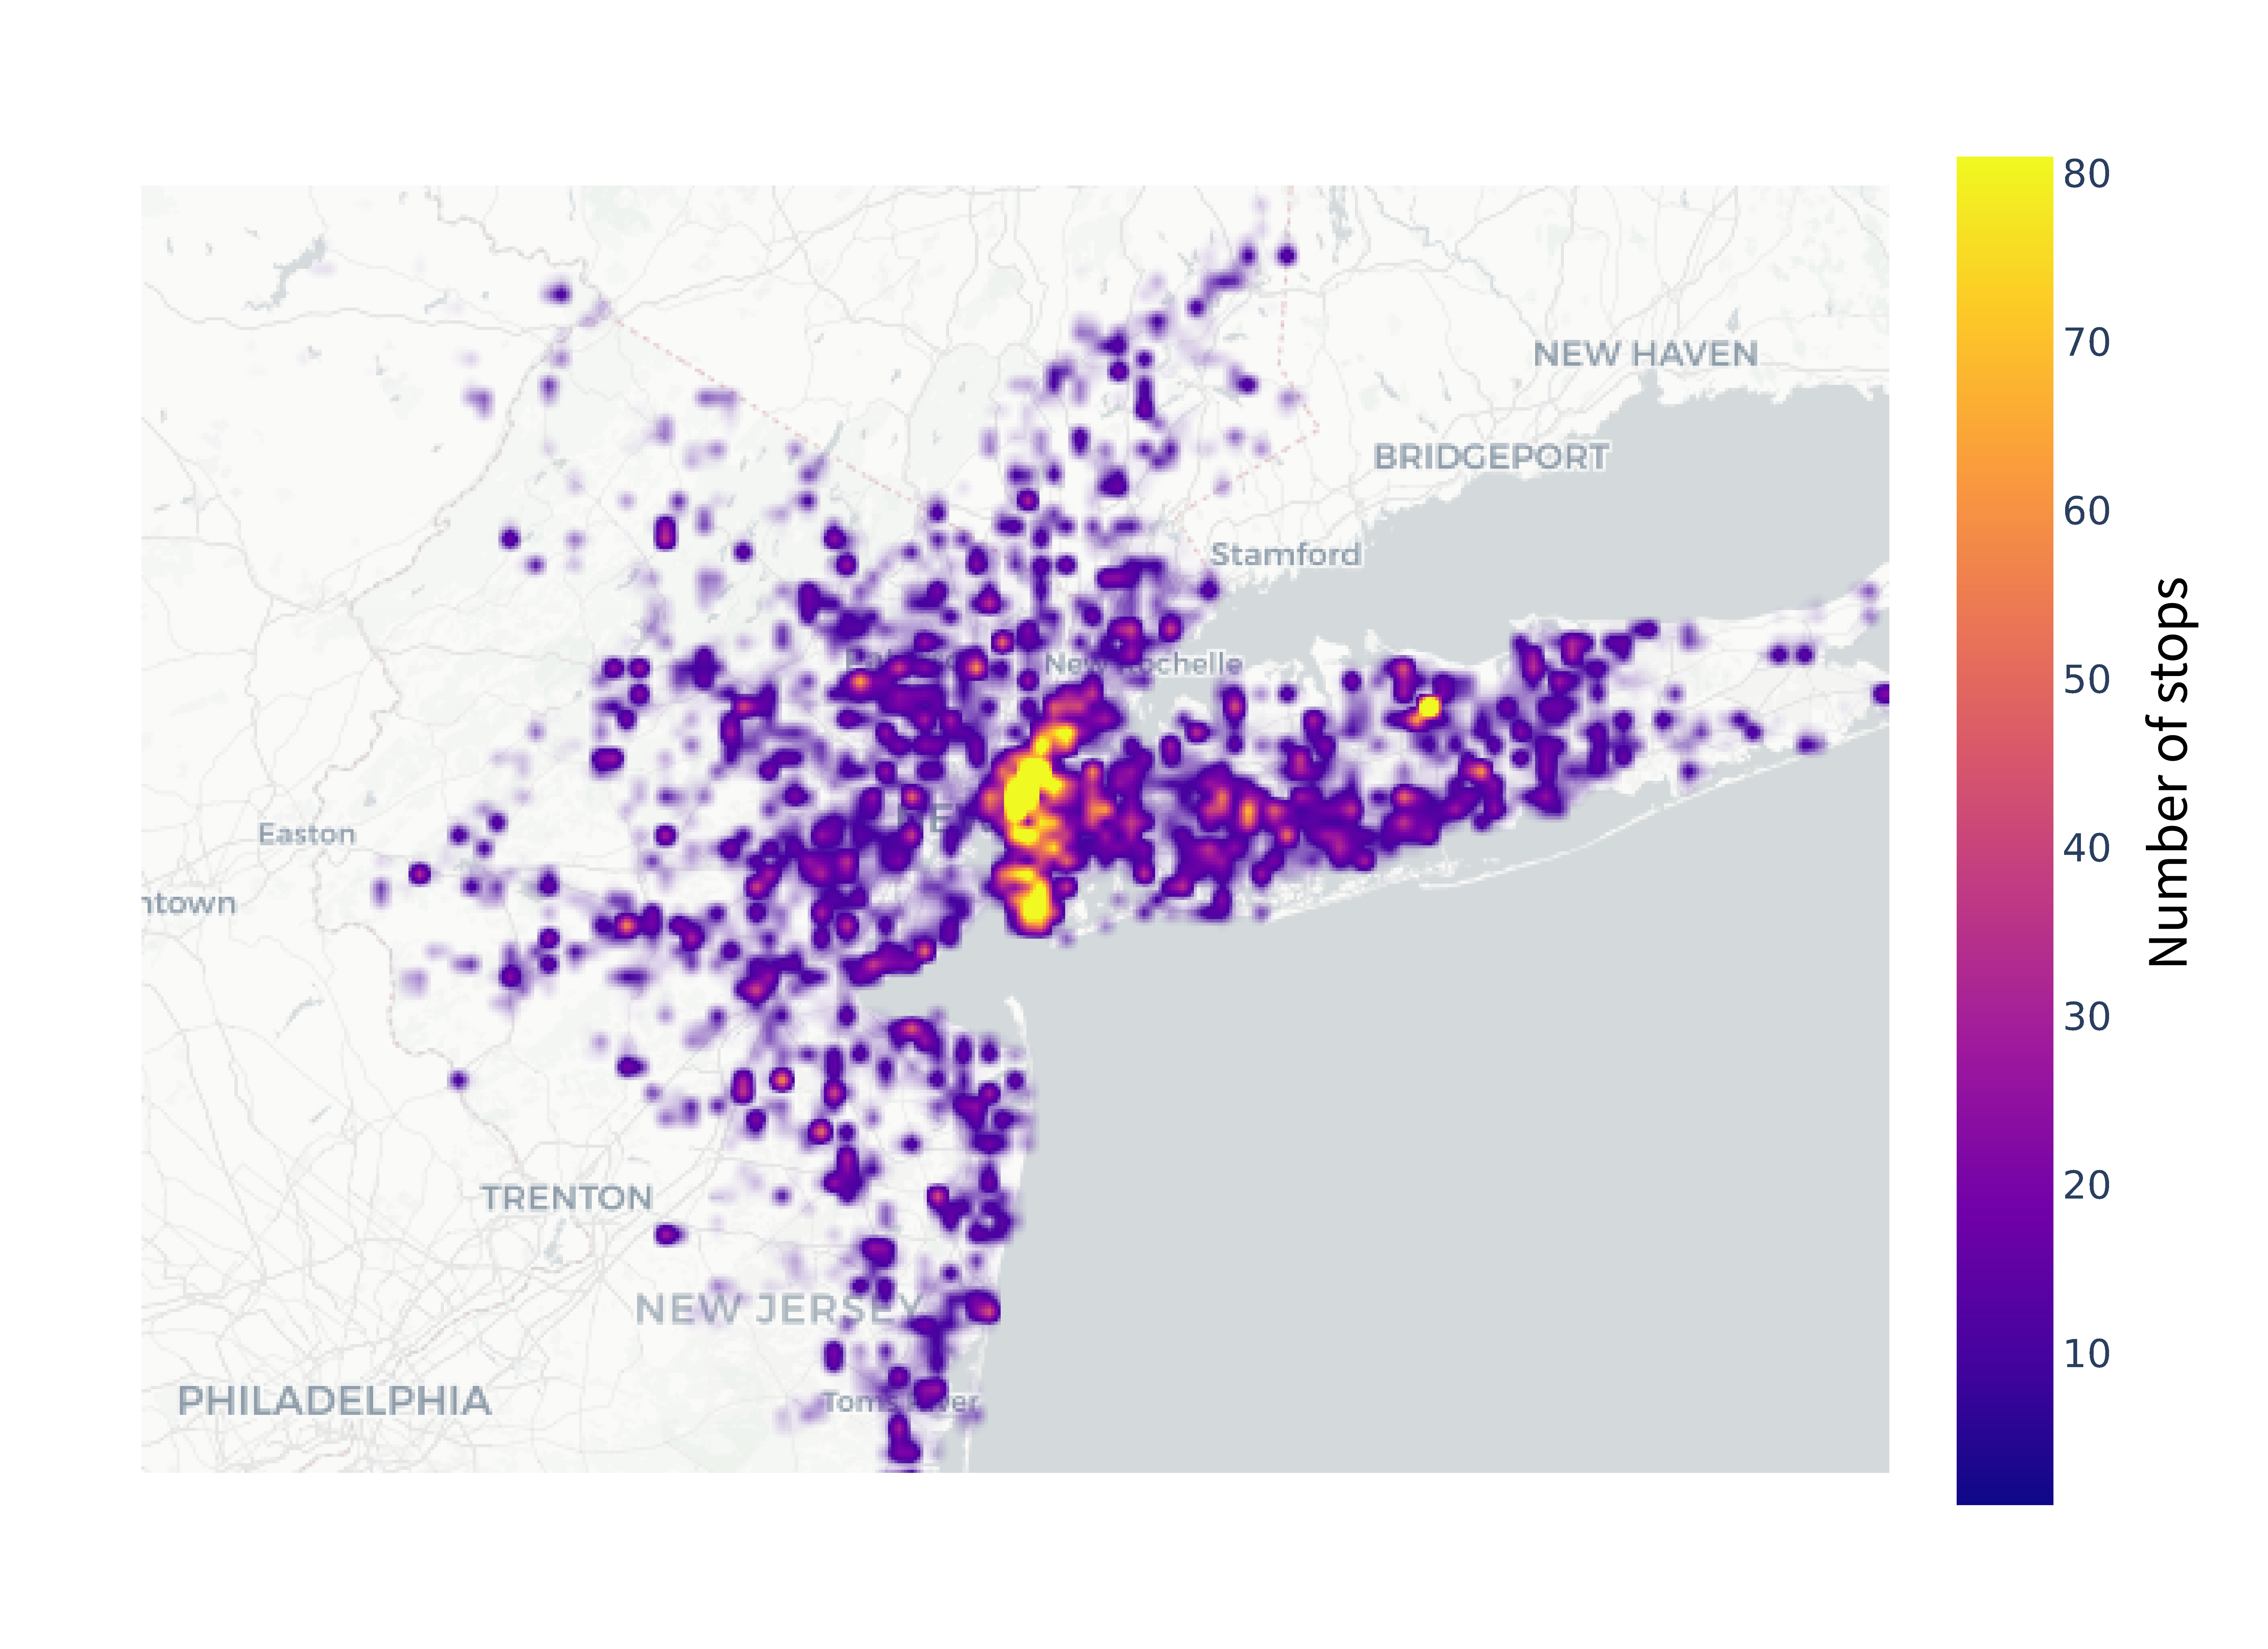
\includegraphics[width=0.8\textwidth]{./Images/heatmap_geohash_all_users.png}
	\centering
	%\fbox{\rule[-.5cm]{4cm}{4cm} \rule[-.5cm]{4cm}{0cm}}
	\caption{Number of stops for each geohash.}
	\label{fig:fig_geohash_heatmap}
\end{figure}




\subsection{Model}
% tell what are the algorithms used (XGBOOST, random forest etc)

\paragraph{Features Engineering}
% add velocity and time interval between data points
We integrated several features drawn from the literature to train the model for detecting stops at points with low data density, all of them are summarized in Table~\ref{tab:feature}.
In line with the approach of leading stop location detection methods, we incorporate two key measurements for each data point to identify its non-stationary characteristics.
The time interval feature for each point is the temporal difference between the timestamps of the previous and the following location for the same device.
The space interval feature for each point is the spatial distance between the positions of the previous and the following location for the same device. It is computed with the haversine formula, which determines the great-circle distance between two points on a sphere given their longitudes and latitudes. 
As suggested in~\citep{Bontorin2024a}, we also integrate individual and collective measures.
At the individual level, we computed the number of stops made by the device in the geohash at level 8 within the past hour, day, and week.
Equivalent metrics are calculated at the community level, analysing collective behaviour within the same geohash area over three different time frames: the previous hour, day and week.
Together with the aforementioned temporal features, we incorporated aggregated data at a specific geographic level (using geohash level 8) for individuals and the community categorized by day of the week and four-hour time blocks (0-3, 4-7, 8-11, 12-15, 16-19, 20-23).
This approach can leverage both personal and collective patterns tied to specific days and periods.


On top of that, we associated each geohash with a measure of entropy to assess the predictability of a geohash in terms of the behaviour of individuals in that location. It is defined as follows.
\begin{equation}
    \label{eq:entropy}
    -\sum_{i=1}^n p_i log (p_i)
\end{equation}
For every geohash, we compute the entropy over total number of devices that stopped (including only geohashes where at least one device stopped). For each device $i$, we compute the probability $p_i$ as the ratio of stops to total passes through the geohash over the entire observation period.
Finally, we incorporated some external information to complement the mobility data.
The classification made by Cuebiq to label the type of data point is assigned according to the following criteria: \textit{whitelisted} is any point that falls within a ``whitelist'' point of interest (POI) included in Cuebiq' POI whitelist,  \textit{personal\_area} are top recurrent area for that device, \textit{blacklisted} are location like hospitals, that are sensitive POI, \textit{other} is any point that does not meet the criteria of the other classifications).
We've added a feature to label the date with a binary holiday indicator, set to 1 for holidays in the relevant geographic area. Additionally, with the accuracy feature, we assess device signal precision using an accuracy measure, representing the circle radius centred in the coordinate pair given by the ping.
Further, for each stop identified by the density-based algorithm, we assign an integer label reflecting the average traffic at that location during the relevant period.

All the numerical features related to the trajectory part are normalized with standard scaler, while we applied one-hot-encoding to categorical non-binary features.


% all the numerical features are normalized, we apply one-hot-encoding to categorical data 

\begin{table}
	\caption{Features summary table}
	\centering
 \begin{scriptsize}
	\begin{tabular}{ll}
 % feat name | description | datatype
		\toprule
		Feature     & Description   \\
		\midrule
	Time interval & Temporal difference between the timestamps of the previous and following locations for each device. \\
		Spatial interval & Spatial distance between the positions of the previous and following locations for each device. \\
		Previous hour individual history &  Individual's stop count in a specific geohash during the previous hour \\
		Previous day individual history     & Individual's stop count in a specific geohash during the previous day  \\
		Previous week individual history     & Individual's stop count in a specific geohash during the previous week  \\
  
		Previous hour geohash collective history & Total stops within a specific geohash during the previous hour \\
		Previous day geohash collective history     & Total stops within a specific geohash during the previous day  \\
		Previous week geohash collective history     & Total stops within a specific geohash during the previous week  \\
  
        %\midrule
		Geohash7 individual history by hour of the day   & Individual's historical stop count in a specific geohash during the same four-hour time window \\
		Geohash7 individual history by day of the week    & Individual's historical stop count in a specific geohash during the same day of the week  \\
  
		Geohash7 collective history by hour of the day   & Total historical stops in a specific geohash during the same four-hour time window  \\
		Geohash7 collective history by day of the week     & Total historical stops in a specific geohash during the same day of the week  \\
  
		Geohash entropy     & Entropy of the distribution of distinct devices per geohash (Eq.~\ref{eq:entropy})\\
  
		Holiday     & Flag (0/1) indicating whether the day is a holiday.  \\
	  Stop type     & Type of stop based on average traffic for the period  \\
	  Accuracy     &  It represents the circle radius centred in the coordinate pair given by the ping \\
	  Point Classification Type     & Classification of the point\\
		\bottomrule
	\end{tabular}
	\label{tab:feature}
 
 \end{scriptsize}
\end{table}




\subsubsection{Validation}
% how we split train and test
We designed the model evaluation framework encompassing a training, test and validation procedure. For this scope, we divided the dataset into training (60\%), test (20\%), and validation (20\%) sets using a temporal ordering to prevent data leakage. The split is based on stop points to ensure each set accurately represents the overall distribution of stops.
The process follows these steps:

\begin{itemize}
    \item We determine a reference date that splits the stop points so 60\% fall before it.
    \item We assign non-stop points to each set based on their timestamp.
    \item To maintain data integrity, we ensure all points from a single stop event are in the same set.    
\end{itemize}

This approach preserves the temporal structure of the data while maintaining representative proportions of stop and non-stop points across all sets.





%60-20-20 temporal split mantenendo l'ordine temporal per evitare data leakage, since the past information is used to determine the features of each point. the split is done considering only the points, such that the percentage of data in each set is representative of the number of stops we have in each. then, for instance, to create the training set we select the date such that the number of stop points before that day is 60\% of the total number of stops. after that, for each set all non-stop points falling in the associated time window are included. finally, we avoid different points representing the same stop belonging to different sets by manually moving them in a single one (to avoid data leaking)
% versione 2: We designed the model test dividing the dataset into training (60\%), test (20\%), and validation (20\%) keeping in the splitting a temporal ordering to prevent data leakage (we want to avoid that points associated to the same stop are divided in different subsets).  To split the entire training set, we selected a reference date such that the number of stops spotted by the density-based algorithm before this date comprises 60\% of the total stops. 
%For each set, we included all non-stop points that fall within the corresponding time window. Additionally, to prevent different points representing the same stop from being in different sets, we manually consolidated them into the same set.




\section{Results and Conclusion}
ff





%\begin{figure}
%	\centering
%	\fbox{\rule[-.5cm]{4cm}{4cm} \rule[-.5cm]{4cm}{0cm}}
%	\caption{Sample figure caption.}
%	\label{fig:fig1}
%\end{figure}



\section{Acknowledgements}
This work is the output of the Complexity72h workshop, held at the Universidad Carlos III de Madrid in Leganés, Spain, 24-28 June 2024. https://www.complexity72h.com

\bibliographystyle{unsrtnat}
\bibliography{references}  %%% Uncomment this line and comment out the ``thebibliography'' section below to use the external .bib file (using bibtex) .


%%% Uncomment this section and comment out the \bibliography{references} line above to use inline references.
% \begin{thebibliography}{1}

% 	\bibitem{kour2014real}
% 	George Kour and Raid Saabne.
% 	\newblock Real-time segmentation of on-line handwritten arabic script.
% 	\newblock In {\em Frontiers in Handwriting Recognition (ICFHR), 2014 14th
% 			International Conference on}, pages 417--422. IEEE, 2014.

% 	\bibitem{kour2014fast}
% 	George Kour and Raid Saabne.
% 	\newblock Fast classification of handwritten on-line arabic characters.
% 	\newblock In {\em Soft Computing and Pattern Recognition (SoCPaR), 2014 6th
% 			International Conference of}, pages 312--318. IEEE, 2014.

% 	\bibitem{keshet2016prediction}
% 	Keshet, Renato, Alina Maor, and George Kour.
% 	\newblock Prediction-Based, Prioritized Market-Share Insight Extraction.
% 	\newblock In {\em Advanced Data Mining and Applications (ADMA), 2016 12th International 
%                       Conference of}, pages 81--94,2016.

% \end{thebibliography}


\end{document}
